% How each experiment script runs (experiments/run_scalability.sh, run_latency.sh, run_ooo_sweep.sh, common.sh).
\documentclass[tikz,border=4pt]{standalone}
\usepackage[T1]{fontenc}
\usepackage{lmodern}
\usetikzlibrary{positioning,fit,arrows.meta,calc,backgrounds}
% Shared look for every diagram. \input this after \usetikzlibrary.
% Greys plus one accent, so the figures print fine in black and white.
\definecolor{accent}{HTML}{2563EB}
\definecolor{accentlight}{HTML}{DBEAFE}
\definecolor{latecol}{HTML}{B45309}
\definecolor{latelight}{HTML}{FEF3C7}
\definecolor{grey}{HTML}{6B7280}
\definecolor{greylight}{HTML}{F3F4F6}
\tikzset{
  box/.style={draw, rounded corners=2pt, align=center, minimum height=7mm, inner sep=3pt, fill=white, font=\footnotesize},
  topic/.style={box, fill=greylight, draw=grey},
  op/.style={box, draw=accent, fill=accentlight},
  ctr/.style={draw=grey, dashed, rounded corners=4pt, inner sep=3mm},
  note/.style={font=\scriptsize, text=grey, align=left},
  arr/.style={-{Latex[length=2mm]}, thick},
  shuffle/.style={arr, double, double distance=0.6pt, -{Latex[length=2.4mm]}},
  latearr/.style={arr, dashed, draw=latecol},
  lbl/.style={font=\scriptsize, fill=white, inner sep=1pt},
}

\tikzset{stp/.style={box, font=\scriptsize, text width=44mm, minimum height=8mm},
         meas/.style={stp, draw=accent, fill=accentlight},
         head/.style={font=\footnotesize\bfseries, align=center, text width=48mm}}
\begin{document}
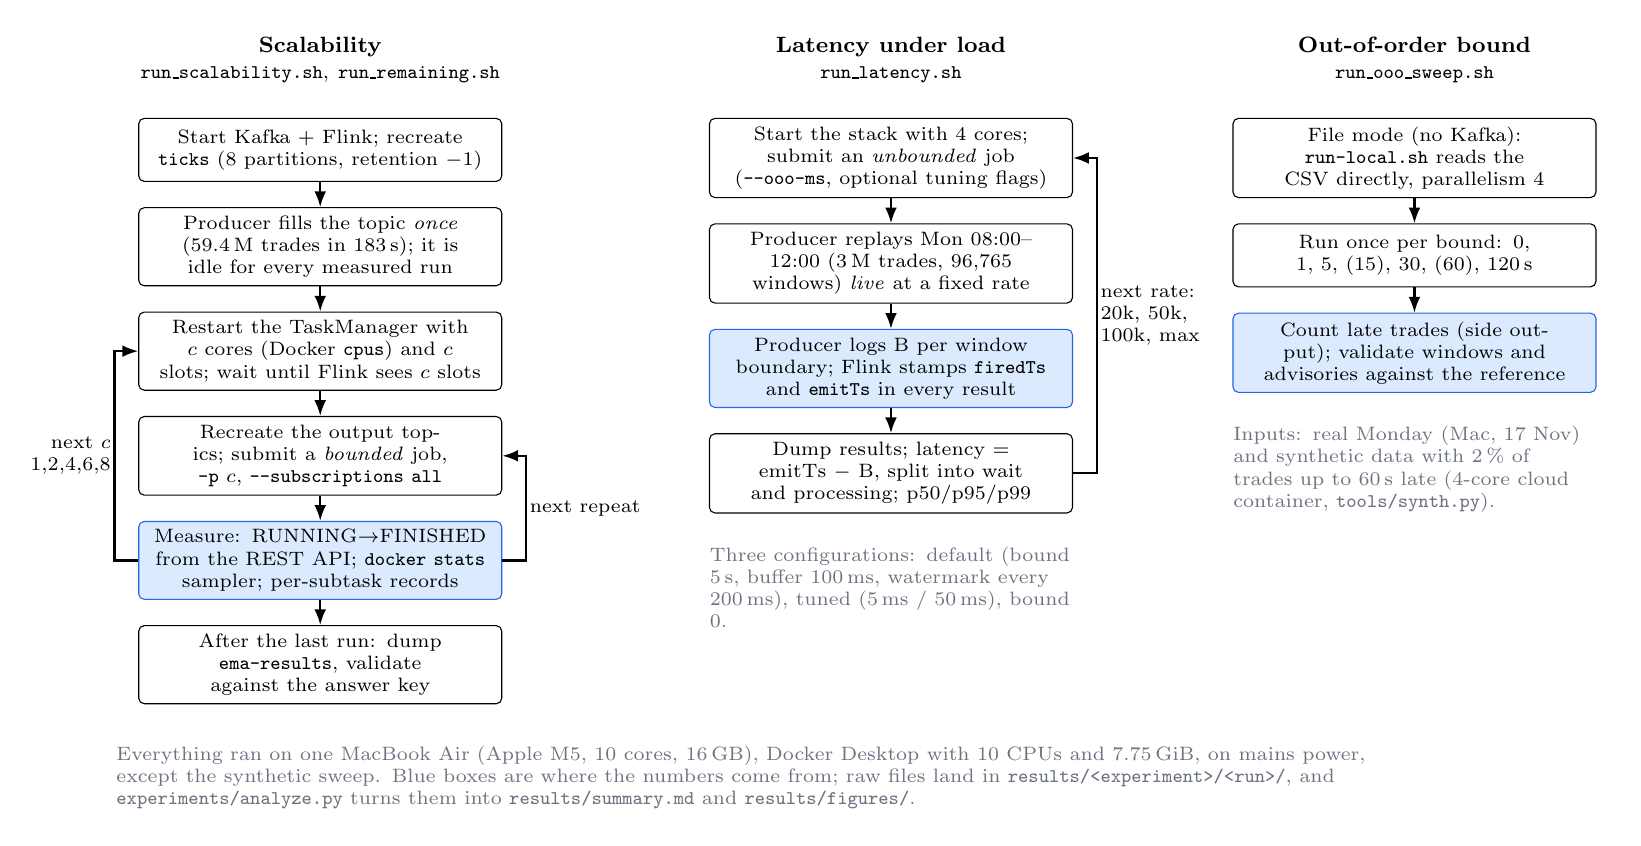
\begin{tikzpicture}[node distance=3.2mm]
  % ---------- scalability
  \node[head] (h1) {Scalability\\\mdseries\scriptsize\texttt{run\_scalability.sh}, \texttt{run\_remaining.sh}};
  \node[stp, below=of h1] (s1) {Start Kafka + Flink; recreate \texttt{ticks} (8 partitions, retention $-1$)};
  \node[stp, below=of s1] (s2) {Producer fills the topic \emph{once} (59.4\,M trades in 183\,s); it is idle for every measured run};
  \node[stp, below=of s2] (s3) {Restart the TaskManager with $c$ cores (Docker \texttt{cpus}) and $c$ slots; wait until Flink sees $c$ slots};
  \node[stp, below=of s3] (s4) {Recreate the output topics; submit a \emph{bounded} job, \texttt{-p} $c$, \texttt{-{}-subscriptions all}};
  \node[meas, below=of s4] (s5) {Measure: RUNNING$\to$FINISHED from the REST API; \texttt{docker stats} sampler; per-subtask records};
  \node[stp, below=of s5] (s6) {After the last run: dump \texttt{ema-results}, validate against the answer key};
  \draw[arr] (s1)--(s2); \draw[arr] (s2)--(s3); \draw[arr] (s3)--(s4); \draw[arr] (s4)--(s5); \draw[arr] (s5)--(s6);
  \draw[arr] (s5.east) -- ++(3mm,0) |- node[lbl, pos=0.25, right, fill=none, align=left]{next repeat} (s4.east);
  \draw[arr] (s5.west) -- ++(-3mm,0) |- node[lbl, pos=0.25, left, fill=none, align=right]{next $c$\\1,2,4,6,8} (s3.west);

  % ---------- latency
  \node[head, right=22mm of h1] (h2) {Latency under load\\\mdseries\scriptsize\texttt{run\_latency.sh}};
  \node[stp, below=of h2] (l1) {Start the stack with 4 cores; submit an \emph{unbounded} job (\texttt{-{}-ooo-ms}, optional tuning flags)};
  \node[stp, below=of l1] (l2) {Producer replays Mon 08:00--12:00 (3\,M trades, 96,765 windows) \emph{live} at a fixed rate};
  \node[meas, below=of l2] (l3) {Producer logs B per window boundary; Flink stamps \texttt{firedTs} and \texttt{emitTs} in every result};
  \node[stp, below=of l3] (l4) {Dump results; latency = emitTs $-$ B, split into wait and processing; p50/p95/p99};
  \draw[arr] (l1)--(l2); \draw[arr] (l2)--(l3); \draw[arr] (l3)--(l4);
  \draw[arr] (l4.east) -- ++(3mm,0) |- node[lbl, pos=0.25, right, fill=none, align=left]{next rate:\\20k, 50k,\\100k, max} (l1.east);
  \node[note, below=3mm of l4, text width=46mm] {Three configurations: default (bound 5\,s, buffer 100\,ms, watermark every 200\,ms), tuned (5\,ms / 50\,ms), bound 0.};

  % ---------- ooo sweep
  \node[head, right=16mm of h2] (h3) {Out-of-order bound\\\mdseries\scriptsize\texttt{run\_ooo\_sweep.sh}};
  \node[stp, below=of h3] (o1) {File mode (no Kafka): \texttt{run-local.sh} reads the CSV directly, parallelism 4};
  \node[stp, below=of o1] (o2) {Run once per bound: 0, 1, 5, (15), 30, (60), 120\,s};
  \node[meas, below=of o2] (o3) {Count late trades (side output); validate windows and advisories against the reference};
  \draw[arr] (o1)--(o2); \draw[arr] (o2)--(o3);
  \node[note, below=3mm of o3, text width=46mm] {Inputs: real Monday (Mac, 17 Nov) and synthetic data with 2\,\% of trades up to 60\,s late (4-core cloud container, \texttt{tools/synth.py}).};

  \node[note, anchor=north west, text width=160mm] at ($(s6.south west)+(-4mm,-4mm)$) {Everything ran on one MacBook Air (Apple M5, 10 cores, 16\,GB), Docker Desktop with 10 CPUs and 7.75\,GiB, on mains power, except the synthetic sweep. Blue boxes are where the numbers come from; raw files land in \texttt{results/<experiment>/<run>/}, and \texttt{experiments/analyze.py} turns them into \texttt{results/summary.md} and \texttt{results/figures/}.};
\end{tikzpicture}
\end{document}
